\section{Method and Data} 
\label{sec:method}
From a holistic view of research method (Figure~\ref{fig:Research Method}), it
consists of three independent but relational parts of the dataset import,
dataset Processing, and machine model training for making binary classifier.

In dataset import process, since the dataset is un-hydrated, we needed
to “hydrate” the data by building a process that will fetch the tweet content
by querying with the Tweet ID. After hydrating, the data are saved in a local
storage, and by using Tweets API the data are completed to be analyzed and
stored in the Elasticsearch server. 
\begin{figure}[h]
\centering
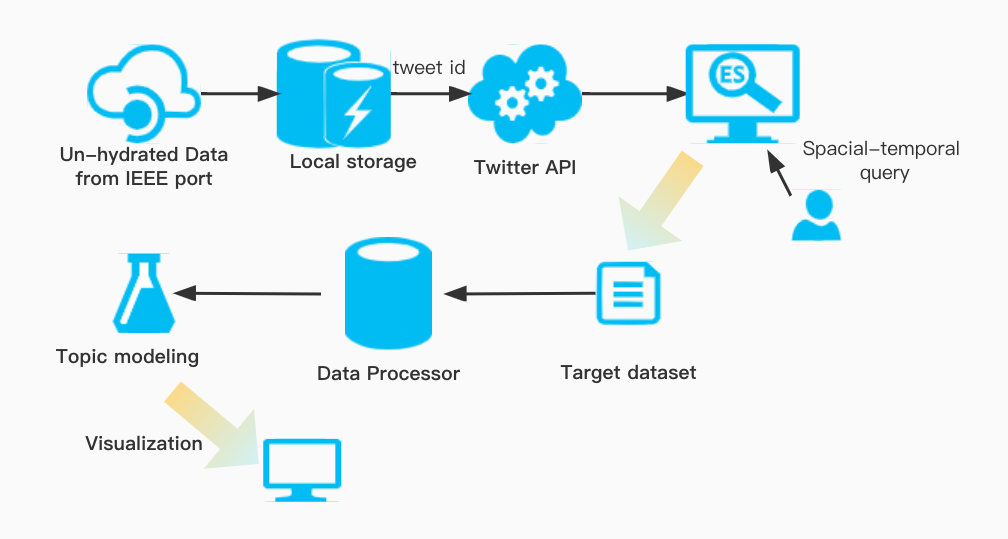
\includegraphics[width=0.5\textwidth]{imgs/freamwork.jpg}
\caption{System structure}
\label{fig:Research Method}
\end{figure}
In dataset processing step, after importing data into Elasticsearch server in
batches, we choose a spatio-temporal research area such
as “7/20/2021-02/01/2022 in California”, and we get the target dataset from
Elasticsearch. By doing spatial query and filtering task, the target dataset
can be visualized into a map. Furthermore, after processing the data by using
techniques such as the regex filtering, tokenization and tagging, and
removing stop words, it is possible to retrieve a word could graph
representing the distribution of keywords according to their degree of
priority.

In model training session, the processed data are delivered to two independent
modules: (a) the binary classifier for sentiment analysis (b) topic
clustering module based on an advanced Deep Learning model architecture such
as the Transformer. To summarize, once the data get processed, they are
applied with the machine learning models to be analyzed.

\subsection{Tweet Data Collection and Processing}
\subsubsection{Tweet Data Collection process}
The dataset we used is CORONAVIRUS (COVID-19) GEO-TAGGED TWEETS DATASET form
IEEE DataPort. Due to the tweets spreading policy. We can't access the
completed tweets content directly.  Thus. We use a transfer program named
Twarc to batch fetch tweets in the dataset. Twarc is a python package
that used to export tweets automatically.  The main principle is that Twarc
will make use of the registration information from twitter developer platform
and get the permission from Twitter. Then Twitter can monitor the whole
process of getting tweets. This way is completely legal and doesn't violate
the privacy protocols set by Twitter. But it also cause some issues. If the
tweets account is banned or the permission has been changed, we can't access
the content anymore. Normally Twitter doesn't send any warning message but
change the content of tweets to a prompt message. So some filtering process
is necessary to ensure that the data set is not contaminated with irrelevant
information. 

We collect data from March 2020 to March 2022. These data comes form hundreds
of single CSV files, Since they are stored by date. So a batch process is
necessary to import from these files. After that we store all of these data
to Elasticsearch, in order to facilitate subsequent steps to call. After
delete all the irrelevant information or the missing information data. The
whole memory size up to 142Mi. The number of useful pieces of information
reaches 388,719. However, the geographical distribution of this tweets is
very uneven. So we try to select states with large sample sizes as research
subjects. 

\subsubsection{Tweet Data structure}
The original data contains tweets ID and sentiment score calculated by
database publisher Figure~\ref{fig:Tweet dataset}. We use tweets ID to
request twitter API in batch and get completed information, including
content, UTC time, geographic location. All of these information are fully
imported into the server after splicing with sentiment score.  In this
process, we will transfer the longitude and latitude to the geometry, then we
can apply some spatial operator to handle them. Time format is another point
in this way, we transfer all the time appearing in our project to UTC format.
Then all filtering of time will be consistent. 
\begin{figure}[h]
\centering
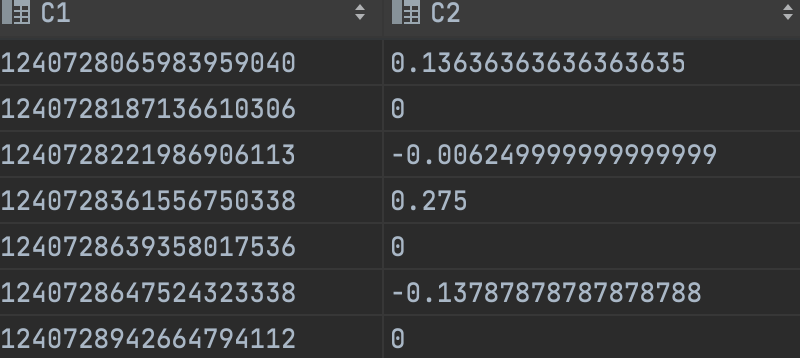
\includegraphics[width=0.5\textwidth]{imgs/row_tweets.png}
\caption{Tweet dataset structure}
\label{fig:Tweet dataset}
\end{figure}
\subsubsection{Tweet Data Pre-processing Method}
The pre-processing process includes regex filtering, tokenization and tagging,
removal of stop words (Figure~\ref{fig:Tokenization and tag}). Regex
filtering process used to delete some proper noun or URL. We can also delete
all the hashtag or the emojis. Normal phrase or locations can also be a
optional. Basically, we will set different filtering rules according to the
task goals and model requirements. 

Tokenization and tag are important to our project. We use nltk package to
process the sentence in the tweets and decompose the content into single
words. Then we can filter for parts of speech and get more reasonable
results. 
\begin{figure}[h]
\centering
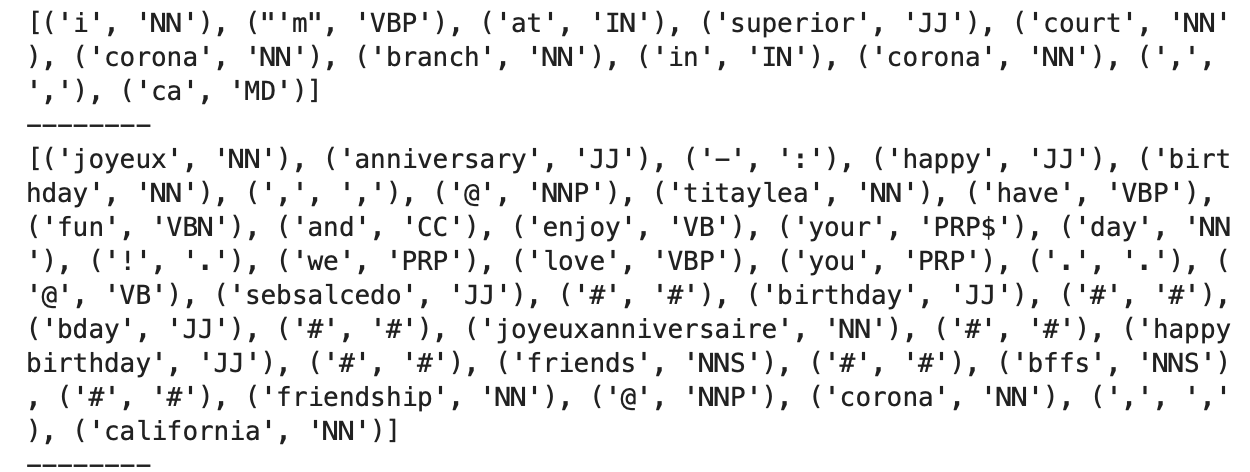
\includegraphics[width=0.5\textwidth]{imgs/tokenization.png}
\caption{Tokenization and tag}
\label{fig:Tokenization and tag}
\end{figure}
The purpose of removal of stopwords is to avoid distractions from common words
on the topic. The nltk package provide a library of stopwords and we can set
our own list of common words based on the theme. It's an important step to
get good performance of machine learning models and we can adjust it to fit
the current strategy we used. It's a part of fine turning. 

\subsection{Topic Clustering}
For topic clustering, first we collected the data from Elasticsearch server by
filtering using spatial queries. The data had text, geo-tag and tweet ID as
data columns. Since the text contained lots of unwanted strings or
characters, we needed to clean the data. 

Some tweet contains hypertext URL such as: 
\begin{verbatim}
    https://t.co/{tweet_id}
\end{verbatim} and some other URLs as shown in (Figure~\ref{fig:Right-most column}):
% \begin{figure}[H]
%     \centering
%     
\includegraphics[width=0.5\textwidth]{url.JPG}
%     \caption{An example of Tweet containing URL}
%     \label{fig:tw_url}
% \end{figure}
    
We needed to filter these unnecessary texts from the actual twitter data using
some regular expression operator and cleaning the part that corresponds to
those specific terms. We also needed to remove all the punctuation marks so
that it drops the redundant and recurring feature that don't contribute to
the clustering.

Example of these regular expression technique is shown in the (Figure~\ref
{fig:Shows the conceptual}): 
\begin{figure}[H]
    \centering
    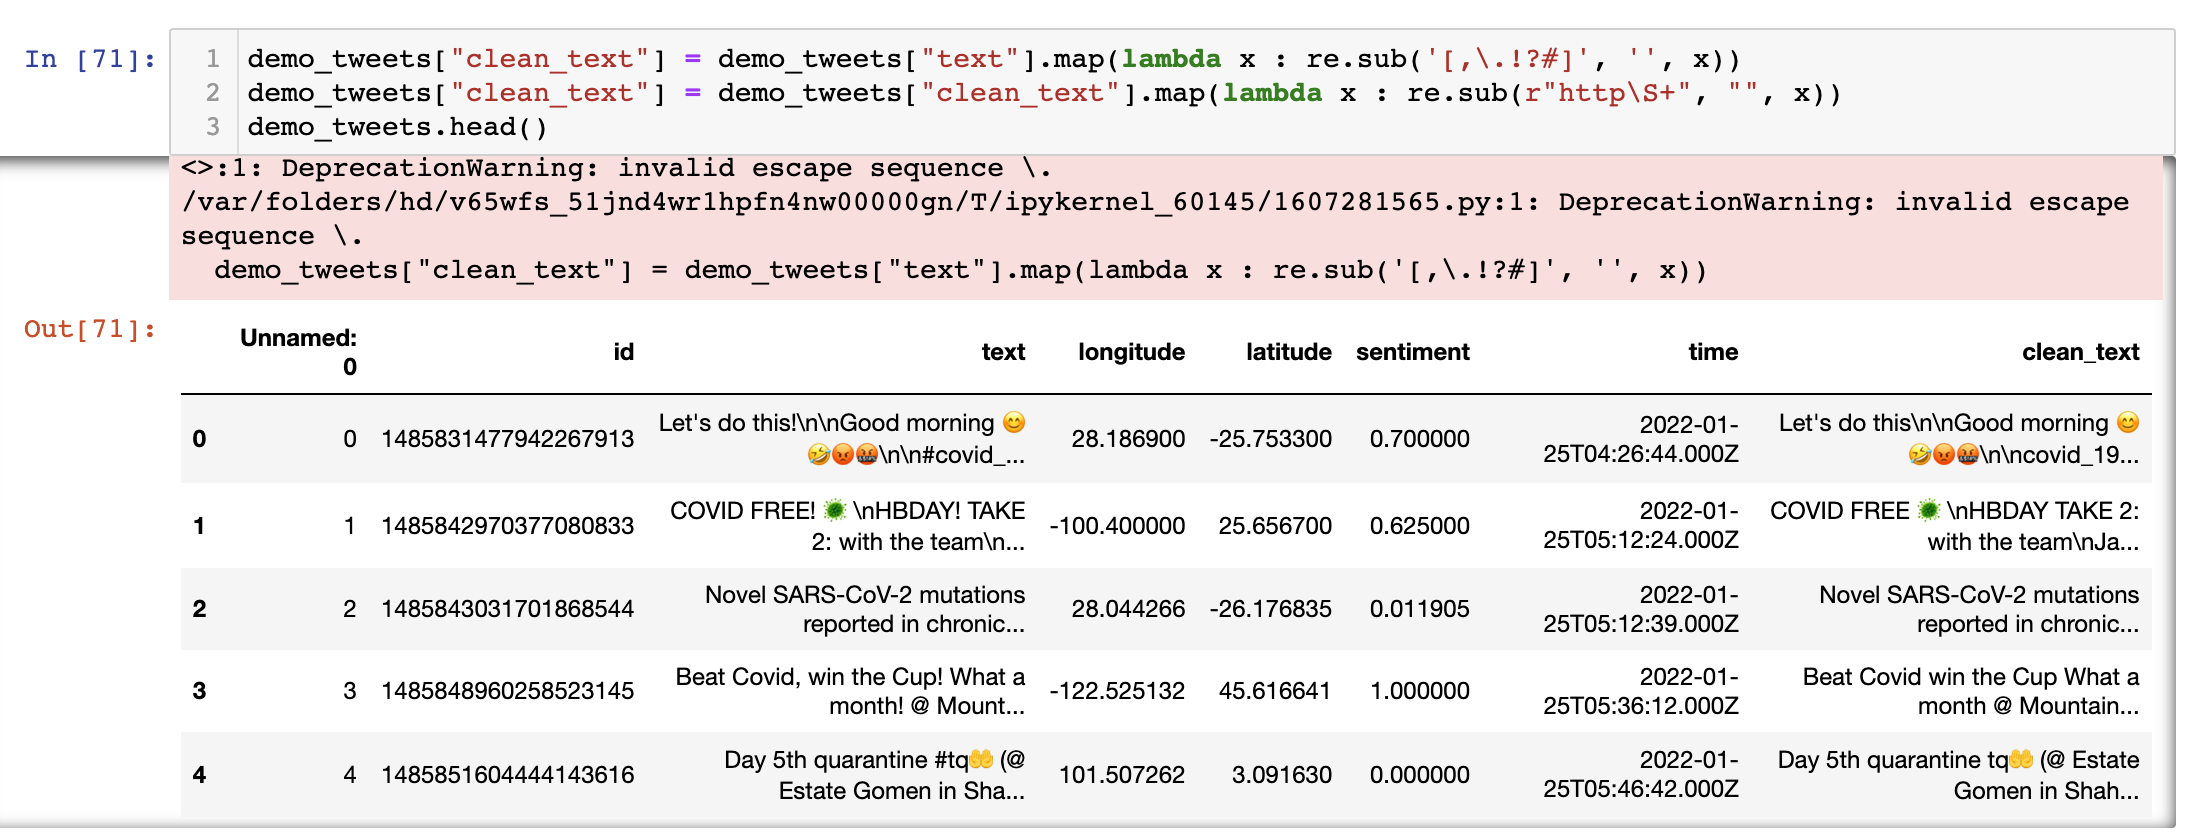
\includegraphics[width=0.5\textwidth]{imgs/cleaning_w_regex.png}
    \caption{Right-most column showing cleaned text with Regex}
    \label{fig:Right-most column}
\end{figure}
After cleaning the data, it was added as a new column in the data frame. The
data frame then was used to generate a word cloud using a Python package
named WordCloud for visualizing the frequency of the terms. Then the data was
processed to remove the English stop words using a library called NLTK which
has available corpus to remove the stop words using the built-in methods. The
reason for cleaning the stop words is to discard them from the consideration
of clustering since those stop words, such as, pronouns, prepositions,
articles are used most frequently and can bias the cluster from finding the
appropriate meaningful terms for the clustered topics. After cleaning the
stopwords, we used a Python package which has built in support for Latent
Dirichlet Allocation. LDA is a popular static technique to find the most
probable terms to determine a topic cluster which describes a subset of
documents in the dataset. Documents can be considered a distribution of
possible topic clusters whereas each topic cluster can be seen as a
distribution of possible terms (words).
\begin{figure}[h]
\centering
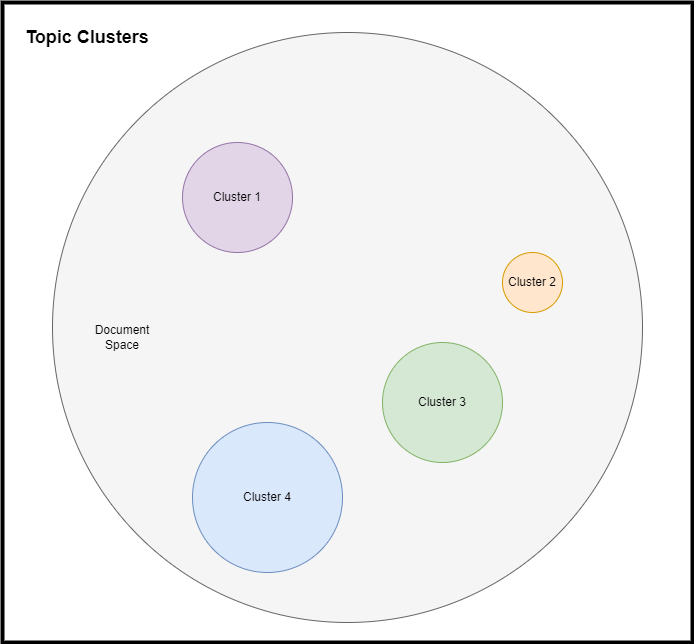
\includegraphics[width=0.5\textwidth]{imgs/topic_clusters.png}
\caption{ Shows the conceptual document space and topic clusters}
\label{fig:Shows the conceptual}
\end{figure}
The size of the circle in (Figure~\ref{fig:Shows the conceptual2}) determines
the number of documents that correspond to the number of clusters. For
example, Cluster 4 shaded in blue has more documents correspondence than
Cluster 3.
\begin{figure}[H]
\centering
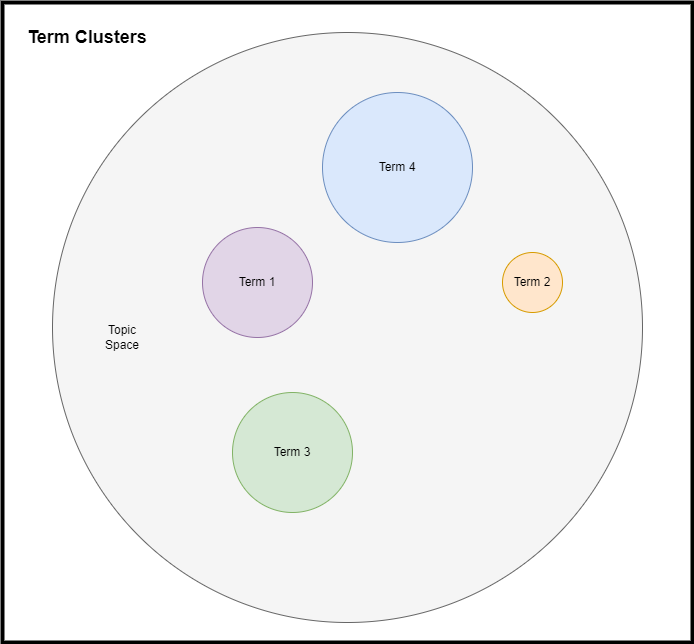
\includegraphics[width=0.5\textwidth]{imgs/term_clusters.png}
\caption{ Shows the conceptual topic space and term clusters}
\label{fig:Shows the conceptual2}
\end{figure}
In the (Figure~\ref{fig:Completed dataset}), the circle size of the term
clusters visualize the frequency of the terms appearing in the documents.

\subsection{Spatial Data Mining and Visualization}
\subsubsection{Data Mining Method}
First, we import all data into Elasticsearch server. Then we get to use
different type of query instructions to request data on demands. In order to
narrow down the scope of our research range, we build two methods and
well-package them, which are query by time and query by location.
Regionally-targeted requests are often broken down by state. So we use two
key steps to accomplish the filtering to the data. First, get the minimum
circumscribed rectangle of the state to search. Next, filter out all points
outside  the boundary by spatial operations. 

\subsubsection{Visualization Method}
We use matplotlib to generate the map automatically. At the same time, we
distinguish different types of points and areas by marking the map with
different colors. Depending on the focus, we'll display a national map or a
state map.